%%%%%%%%%%%%%%%%%%%%%%%%%%%%%%%%%%%%%%%%%%%%%%%%%%%%%%
% A Beamer template for Ritsumeikan University       %
% Author: Ming-Hao Xu (Xu Minghao)                   %
% Date:   April 2022.                                %
% LPPL Licensed.                                     %
%%%%%%%%%%%%%%%%%%%%%%%%%%%%%%%%%%%%%%%%%%%%%%%%%%%%%%

\documentclass{beamer}
\usepackage{hyperref}

\usepackage[UTF8]{ctex}
\usepackage[T1]{fontenc}

% other packages
\usepackage{latexsym,amsmath,xcolor,multicol,booktabs,calligra}
\usepackage{graphicx,pstricks,listings,stackengine}
\usefonttheme[onlymath]{serif}

% dummy text; remove it when working on this template
\usepackage{lipsum}

\author{Ebola}
\title{计算几何3:半平面交、随机增量法}
\institute{
    Institute of Mathematics, \\
    Zhejiang University.
}
\date{Jan, 2024}
\usepackage{Ritsumeikan}

% defs
\def\cmd#1{\texttt{\color{red}\footnotesize $\backslash$#1}}
\def\env#1{\texttt{\color{blue}\footnotesize #1}}
\definecolor{deepblue}{rgb}{0,0,0.5}
\definecolor{deepred}{rgb}{0.6,0,0}
\definecolor{deepgreen}{rgb}{0,0.5,0}
\definecolor{halfgray}{gray}{0.55}

\lstset{
    basicstyle=\ttfamily\tiny,
    keywordstyle=\bfseries\color{deepblue},
    emphstyle=\ttfamily\color{deepred},    % Custom highlighting style
    stringstyle=\color{deepgreen},
    numbers=left,
    numberstyle=\small\color{halfgray},
    rulesepcolor=\color{red!20!green!20!blue!20},
    frame=shadowbox,
}


\begin{document}

\begin{frame}
    \titlepage
\end{frame}

\begin{frame}
    \tableofcontents[sectionstyle=show,subsectionstyle=show/shaded/hide,subsubsectionstyle=show/shaded/hide]
\end{frame}

\section{半平面交}

\begin{frame}{基础回顾:直线求交}
    \small
    给定两条直线,均用两点式存储。求交点。

    \vspace{1em}\pause
    \begin{figure}[H]
        \centering
        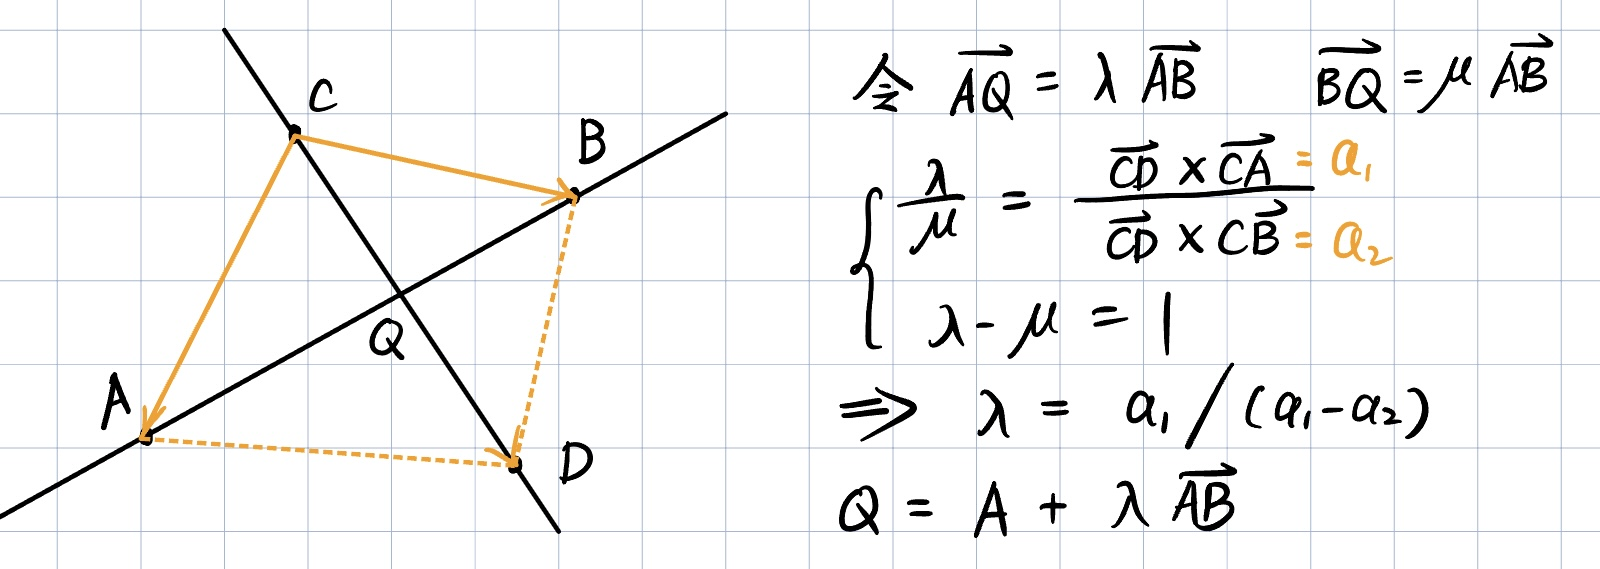
\includegraphics[width=\textwidth]{pic/lineinsect.jpg}
    \end{figure}
\end{frame}

\begin{frame}{半平面交}
    \small
    一条直线可以将平面分成两个部分,
    每个部分都是一个“半平面”。

    \vspace{1em}
    “半平面交”,顾名思义就是很多个半平面相交的部分。
    这个区域有可能是无界的,也有可能是有界的。

    \begin{figure}[H]
        \centering
        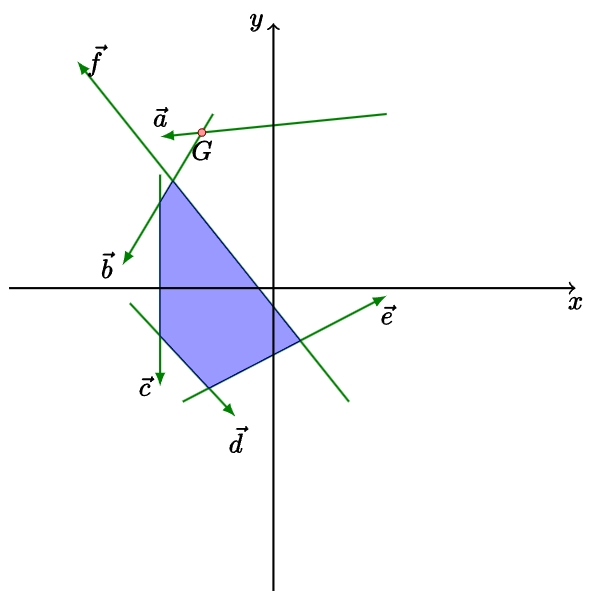
\includegraphics[width=0.5\textwidth]{pic/halfplane_2.png}
    \end{figure}
\end{frame}

\begin{frame}{[CQOI2006] 凸多边形}
    \small
    给定若干个凸多边形(顶点按逆时针顺序给出),
    求所有凸多边形相交区域的面积。

\end{frame}

\begin{frame}[fragile]{半平面交}
    \small
    我们用“有源向量”的形式来储存直线,即保存直线上某一个点(源点)坐标、直线的方向向量。

    \vspace{1em}
    为了方便,我们站在源点,面朝有源向量所指的方向,将左手侧的区域
    称为这个有源向量的“左半平面”。凸多边形的交其实就是很多个
    有源向量的左半平面之交。

    \vspace{1em}
    首先按极角从小到大将所有的有源向量排序,极角可以通过 \verb|atan2(y,x)| 计算,
    该函数返回一个 $\theta\in(-\pi,\pi],\;\theta=\text{arctan}\frac{y}{x}$.

    如果有极角相同的两个有源向量,我们只保留靠左侧的一个。
\end{frame}

\begin{frame}[fragile]{半平面交}
    \footnotesize
    半平面交是一个凸多边形,所以要维护一个凸壳。
    并保存凸壳上的所有顶点。
    新加入一个有源向量 $\overrightarrow{c}$ 时,
    可能会出现下图所示的情况。

    \begin{figure}[H]
        \centering
        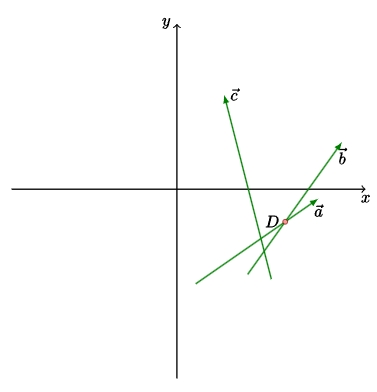
\includegraphics[width=0.4\textwidth]{pic/halfplane_1.png}
    \end{figure}

    此时为了维护凸壳,要把 $\overrightarrow{b}$ 以及交点 $D$ 弹出。
    需要一直弹出,直到最后两条直线的交点在 $\overrightarrow{c}$ 左侧为止。

    \pause
    \begin{lstlisting}[language=c++]
while(!vertex_que.empty() && !l[i].onleft(vertex_que.back()))
    vertex_que.pop_back(), line_que.pop_back();
    \end{lstlisting}
\end{frame}

\begin{frame}[fragile]{半平面交}
    \footnotesize
    现在继续加入有源向量 $\overrightarrow{f}$,
    还有可能会出现下图所示的情况:

    \begin{figure}[H]
        \centering
        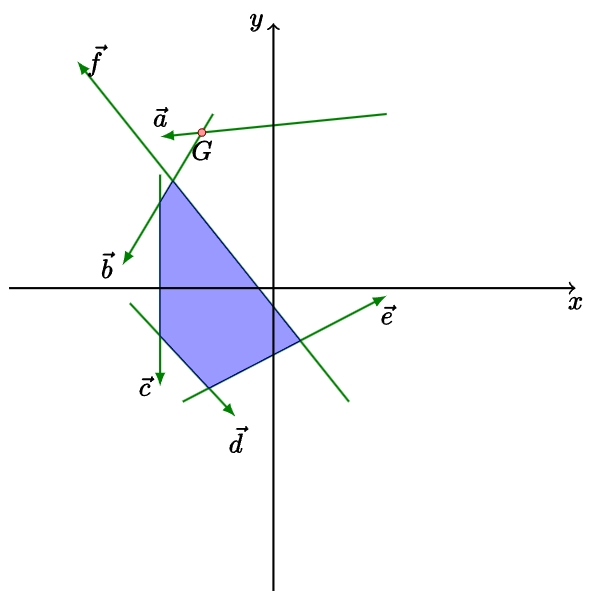
\includegraphics[width=0.4\textwidth]{pic/halfplane_2.png}
    \end{figure}

    即,一开始加入的两条直线的交点 $G$ 落在了 $\overrightarrow{f}$ 右侧。
    此时要从头开始,弹出 $\overrightarrow{a}$ 以及交点 $G$,一直重复,直到最前面
    两条直线的交点在 $\overrightarrow{f}$ 左侧为止。
    
    \pause
    \begin{lstlisting}[language=c++]
while(!vertex_que.empty() && !l[i].onleft(vertex_que.front()))
    vertex_que.pop_front(), line_que.pop_front();
    \end{lstlisting}
\end{frame}

\begin{frame}[fragile]{半平面交}
    \footnotesize
    现在所有的有源向量都已经加入完毕了,
    但是可能会出现下图所示的情况:

    \begin{figure}[H]
        \centering
        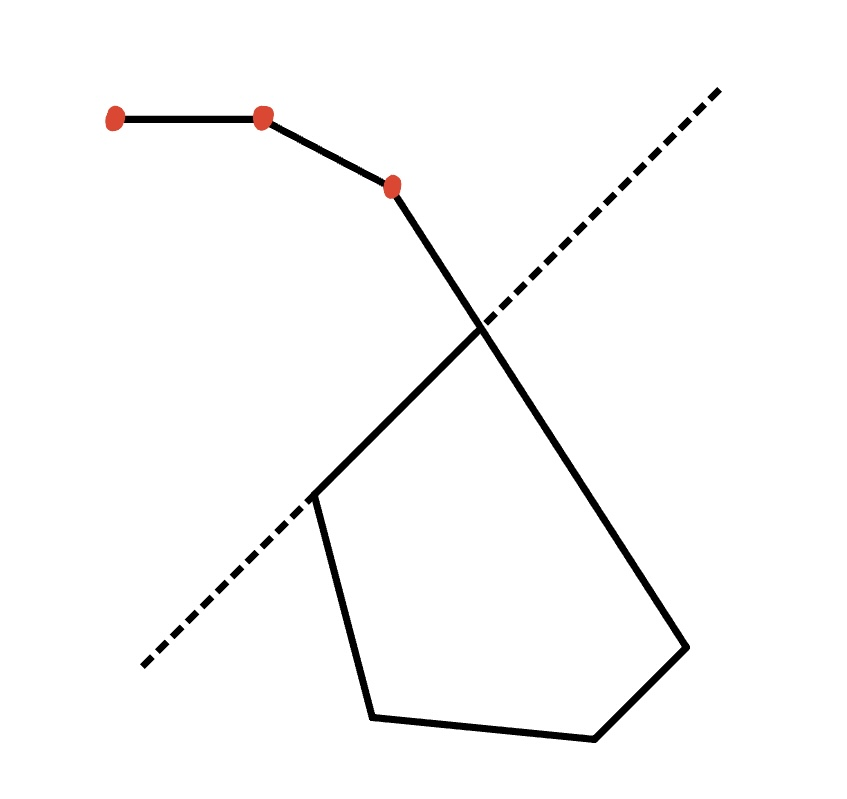
\includegraphics[width=0.35\textwidth]{pic/halfplane_3.jpg}
    \end{figure}

    显然,虚线以上的部分是需要弹出的,我们可以借助
    第一个有源向量来判断,即:若末端的点不在第一个有源向量左侧,
    则弹出,直到末端的点在其左侧为止。

    \pause
    \begin{lstlisting}[language=c++]
while(!vertex_que.empty() && !line_que.front().onleft(vertex_que.back()))
    vertex_que.pop_back(), line_que.pop_back();
// 若只剩一条直线,说明半平面交为空;否则,求出第一条和最后一条直线的交点
if(line_que.size() == 1) return 0;
vertex_que.push_back(line_que.back().crosspoint(line_que.front()));
    \end{lstlisting}
\end{frame}

\begin{frame}[fragile]{半平面交}
    \footnotesize
    完整代码(不含排序和去重):

    \begin{lstlisting}[language=c++]
deque<Line> line_que;
deque<Point> vertex_que;

line_que.push_back(l[0]);
line_que.push_back(l[1]);
vertex_que.push_back(l[0].crosspoint(l[1]));

for(int i = 2; i < tot; i++){
    while(!vertex_que.empty() && !l[i].onleft(vertex_que.back()))
        vertex_que.pop_back(), line_que.pop_back();
    while(!vertex_que.empty() && !l[i].onleft(vertex_que.front()))
        vertex_que.pop_front(), line_que.pop_front();
    vertex_que.push_back(l[i].crosspoint(line_que.back()));
    line_que.push_back(l[i]);
}
while(!vertex_que.empty() && !line_que.front().onleft(vertex_que.back()))
    vertex_que.pop_back(), line_que.pop_back();
vertex_que.push_back(line_que.back().crosspoint(line_que.front()));
    \end{lstlisting}
\end{frame}

\begin{frame}{[POJ 2451] Uyuw's Concert}
    \small
    按逆时针顺序给定多边形的顶点坐标(不一定是凸多边形),
    求多边形内部能够看到所有顶点的区域的面积。(即:多边形的核)

    \vspace{1em}\pause
    【解】其实就是求多边形所有边左侧的半平面交。
\end{frame}

\begin{frame}{ [HNOI2008] 水平可见直线}
    \small
    在 $x-y$ 直角坐标平面上有 $n$ 条直线 $L_1,L_2,…L_n$,若在 $y$ 值为正无穷大处往下看,能见到 $L_i$ 的某个子线段,则称 $L_i$ 为可见的,否则 $L_i$ 为被覆盖的。
例如,对于直线:
$L_1:y=x$;
$L_2:y=-x$;
$L_3:y=0$;
则 $L_1$ 和 $L_2$ 是可见的,$L_3$ 是被覆盖的。给出 $n$ 条直线,表示成 $y=Ax+B$ 的形式($|A|,|B| \le 500000$),且 $n$ 条直线两两不重合,求出所有可见的直线。
\end{frame}

\begin{frame}{ [HNOI2008] 水平可见直线}
    \footnotesize
    显然,从上往下看能看到的部分一定长这样(图片来自洛谷题解):
    \begin{figure}[H]
        \centering
        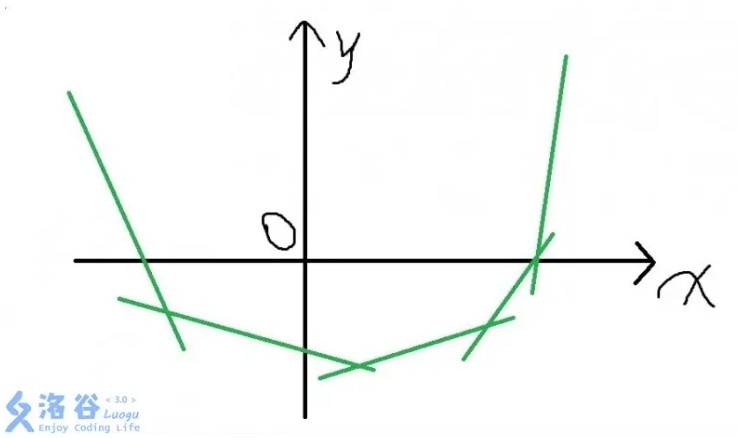
\includegraphics[width=0.7\textwidth]{pic/hnoi2008.png}
    \end{figure}

    所以把每条直线的上侧做半平面交即可。
    要记录一下哪些直线在半平面交里。

    \vspace{1em}
    注意,这题的半平面交是无界的,但我们的算法其实要有界才能跑下去。
    我们可以加上一条非常远的直线来确保有界,同时不影响答案。

    \vspace{1em}\pause
    其实这个题不需要半平面交,维护一个斜率的单调栈也能做。
\end{frame}

\begin{frame}{[SCOI2015] 小凸想跑步}
    \small
    小凸晚上喜欢到操场跑步,今天他跑完两圈之后,他玩起了这样一个游戏。

    操场是个凸 $n$ 边形, $n$ 个顶点按照逆时针从 $0$ ∼ $n - 1$ 编号。现在小凸随机站在操场中的某个位置,标记为 $p$ 点。将 $p$ 点与 $n$ 个顶点各连一条边,形成 $n$ 个三角形。如果这时 $p$ 点, $0$ 号点, $1$ 号点形成的三角形的面
    积是 $n$ 个三角形中最小的一个,小凸则认为这是一次正确站位。
    
    现在小凸想知道他一次站位正确的概率(即符合条件的区域面积占总面积的比)是多少。
\end{frame}

\begin{frame}{[SCOI2015] 小凸想跑步}
    \small
    记第 $i$ 个顶点坐标为 $(x_i,y_i)$,问题可以转化为:
    \begin{equation}
        (y_1-y_0-y_{i+1}+y_i)x + (x_0-x_1+x_{i+1}-x_i)y + (x_iy_{i+1}-x_{i+1}y_i-x_0y_1+x_1y_0) > 0
    \end{equation}
    对所有 $i=1,...,n-1$ 均成立(当 $i=n-1$ 时,$i+1$ 用 $0$ 代替)。

    \vspace{1em}
    把半平面的解析表达式转换成“有源向量左半平面”的表示形式,然后求半平面交即可。
    另外还要记得 $(x,y)$ 必须在凸多边形内部,所以凸多边形的边也要加进来一起做半平面交。
\end{frame}

\begin{frame}{[SDOI2013] 逃考}
    \footnotesize
    \begin{figure}[H]
        \centering
        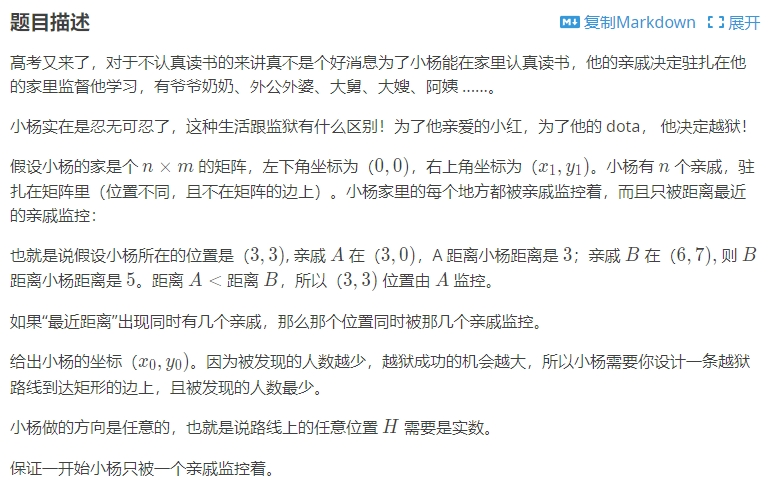
\includegraphics[width=\textwidth]{pic/sdoi2013_prb.png}
    \end{figure}
    \vspace{-1em}
    亲戚数量 $\leq 600$.
\end{frame}

\begin{frame}{[SDOI2013] 逃考}
    \footnotesize
    显然,每个亲戚监控的区域是连通的。
    所以在最优路径下,每跨越一个区域,就会
    多被一个亲戚监控,不会出现跨出去又跨回来的现象。

    \vspace{1em}\pause
    我们可以把每个亲戚监控的区域当成一个点,
    若两个区域相邻,对应的两个点之间就连一条边权为 $1$ 的无向边。
    若区域和边界相邻,则与终点连一条边权为 $1$ 的无向边。
    然后跑最短路即可。

    \vspace{1em}
    现在问题是如何判断两个亲戚的监控区域是否相邻。
\end{frame}

\begin{frame}{[SDOI2013] 逃考}
    \footnotesize
    事实上,亲戚 $A$ 与其它任一亲戚的监控范围,由它们连线的中垂线分开。
    将这些中垂线靠近亲戚 $A$ 一侧的半平面求交,
    就得到了亲戚 $A$ 的监控范围,同时也求出了
    和 $A$ 监控范围相邻的亲戚。

    \begin{figure}[H]
        \centering
        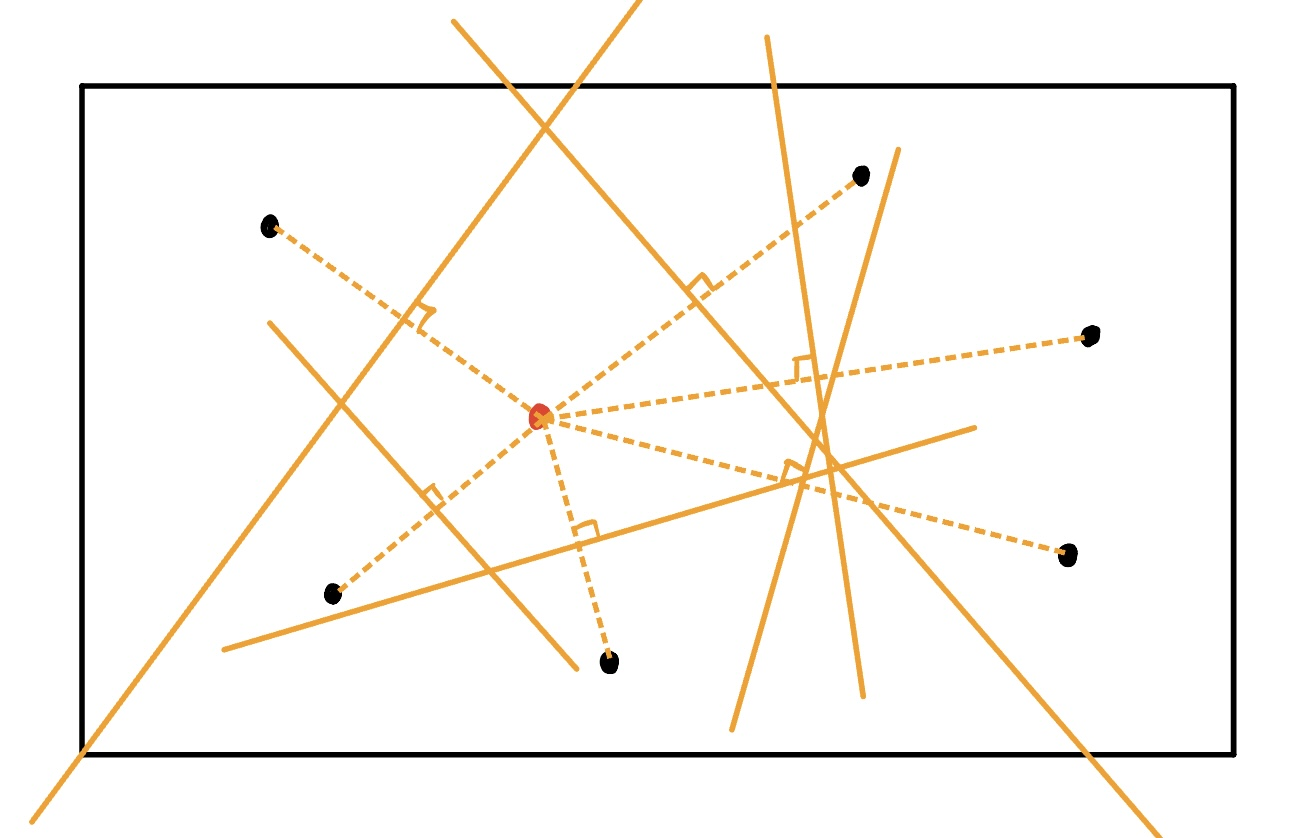
\includegraphics[width=0.7\textwidth]{pic/sdoi2013_sol.jpg}
    \end{figure}

    别忘了还要把矩形的边界加入半平面交。
\end{frame}

\begin{frame}{[HNOI2012] 射箭}
    \small
    给定若干个竖直线段,如果有一条过原点的抛物线 $y=ax^2+bx\;(a<0,b>0)$ 能同时经过
    前 $i$ 条线段,则可以通过第 $i$ 关。问最多能通过几关。

    \vspace{1em}
    线段的数量不超过 $10^5$ 条。
    \begin{figure}[H]
        \centering
        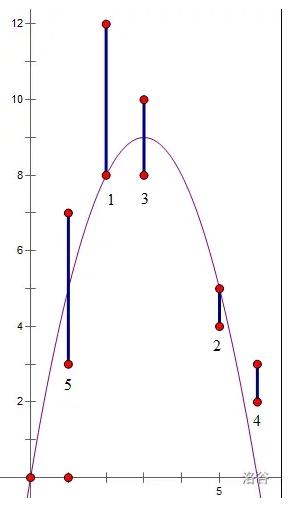
\includegraphics[width=0.3\textwidth]{pic/hnoi2012.png}
    \end{figure}
\end{frame}

\begin{frame}{[HNOI2012] 射箭}
    \footnotesize
    显然,如果能通过第 $i$ 关,就一定可以通过前 $i$ 关。
    所以可以二分答案。接下来就是判断能否通过第 $i$ 关。

    \vspace{.5em}\pause
    设抛物线为 $y=ax^2+bx$,第 $i$ 条线段的横坐标为 $x_i$,
    纵坐标为 $l_i$ 到 $r_i$。那么,第 $i$ 条线段对抛物线的约束为:
    \begin{align}
        ax_i^2 + bx_i &\geq l_i,\\
        ax_i^2 + bx_i &\leq r_i.
    \end{align}

    \vspace{.5em}\pause
    我们把 $(a,b)$ 放在平面上,
    上面的式子其实就是把 $(a,b)$ 约束在了一个半平面中。
    只需要判断半平面交是否非空即可。

    \vspace{.5em}\pause
    \textbf{注记1}:注意不要在检查答案 $mid$ 的时候排序去重,这样会变成两个 $\log$,
    这题比较卡常,过不去。应该先排序(但不能去重),每条直线标记一下编号,
    检查的时候先去重然后求半平面交,碰到编号大于 $mid$ 的直线就跳过。如果
    常数实在太大,可以考虑手写双端队列。

    \textbf{注记2}:不要忘记 $a<0$ 和 $b>0$;另外为了保证半平面交有界,
    我们要在非常左、非常上的地方各加一条边界线;本题卡精度到令人发指,祝诸君顺利!
\end{frame}

\section{随机增量法}

\begin{frame}{最小圆覆盖 (P1743)}
    给定平面上若干个点,求能覆盖所有点的最小圆。
\end{frame}

\begin{frame}{最小圆覆盖}
    \footnotesize
    \textbf{定理1}:最小圆覆盖存在且唯一。

    \vspace{1em}\pause
    \textbf{定理2}:最小圆要么是以某两个点为直径的圆,
    要么是某三个点的外接圆。

    \vspace{1em}\pause
    \textbf{定义}:我们记 $\text{MC}(P_1,...,P_k;Q_1,...,Q_n)$ 表示
    $P_1,...,P_k,Q_1,...,Q_n$ 的最小圆覆盖,其中 $P_1,...,P_k$ 在圆周上。

    \vspace{1em}\pause
    \textbf{引理1}:若 $Q_n\notin \text{MC}(\varnothing;Q_1,...,Q_{n-1})$,那么
    \begin{equation*}
        \text{MC}(\varnothing;Q_1,...,Q_{n})=\text{MC}(Q_n;Q_1,...,Q_{n-1}).
    \end{equation*}

    \vspace{1em}\pause
    \textbf{引理2}:若 $Q_n\notin \text{MC}(P_1;Q_1,...,Q_{n-1})$,那么
    \begin{equation*}
        \text{MC}(P_1;Q_1,...,Q_{n})=\text{MC}(P_1,Q_n;Q_1,...,Q_{n-1}).
    \end{equation*}

    \vspace{1em}\pause
    \textbf{引理3}:若 $Q_n\notin \text{MC}(P_1,P_2;Q_1,...,Q_{n-1})$,那么
    \begin{equation*}
        \text{MC}(P_1,P_2;Q_1,...,Q_{n})=\text{MC}(P_1,P_2,Q_n;Q_1,...,Q_{n-1}).
    \end{equation*}
\end{frame}

\begin{frame}{最小圆覆盖}
    \footnotesize
    \textbf{引理1}:若 $Q_n\notin \text{MC}(\varnothing;Q_1,...,Q_{n-1})$,那么
    \begin{equation*}
        \text{MC}(\varnothing;Q_1,...,Q_{n})=\text{MC}(Q_n;Q_1,...,Q_{n-1}).
    \end{equation*}

    \vspace{1em}
    \textbf{证明}:若不然,我们令当前圆为 $\text{MC}(\varnothing;Q_1,...,Q_{n-1})$,
    让它逐渐变换为 $\text{MC}(\varnothing;Q_1,...,Q_{n})$,过程如下:
    \begin{enumerate}
        \item 逐渐增大半径,直到与 $\text{MC}(\varnothing;Q_1,...,Q_{n})$ 大小相同;
        \item 逐渐平移到 $\text{MC}(\varnothing;Q_1,...,Q_{n})$ 的位置。
    \end{enumerate} 

    \pause 在第一过程中,原来在圆内的点一直还在圆内;
    在第二过程中,不可能有原来的点跑出去,否则它就不会再进来了,从而与
    “覆盖”性质矛盾。

    \pause 但是在第一或第二过程中,一定会有某个时刻,圆周刚好碰到 $Q_n$;
    这时候当前圆是一个半径不超过 $\text{MC}(\varnothing;Q_1,...,Q_{n})$ 的圆覆盖,
    且不同于 $\text{MC}(\varnothing;Q_1,...,Q_{n})$;
    这与最小圆覆盖的唯一性矛盾!

    \vspace{1em}
    引理2、引理3的证明类似(课上有时间可以证一下)。
\end{frame}

\begin{frame}{随机增量法}
    \small
    现在我们有了理论基础,接下来用随机增量法来求解最小圆覆盖。

    \vspace{1em}\pause
    “增量法”的意思是将一个问题化为规模刚好小一层的子问题。
    解决子问题后加入当前的对象。

    \vspace{1em}\pause
    具体来说,在最小圆覆盖问题中,就是
    先解决前 $i$ 个点的最小圆覆盖,
    然后加入第 $i+1$ 个点,并修正答案;
    一直到加完所有点为止。

    \vspace{1em}\pause
    “随机增量法”就是先把所有点的顺序打乱,
    然后做“增量法”。
\end{frame}

\begin{frame}[fragile]{随机增量法}
    \footnotesize
    我们用增量法来求 $\text{MC}(\varnothing;Q_1,...,Q_{n})$,即
    从 $\text{MC}(\varnothing;Q_1)$ 开始,逐渐增加 $Q_2,...,Q_{n-1}$。

    \vspace{1em}\pause
    假设现在已经有了 $\text{MC}(\varnothing;Q_1,...,Q_{i-1})$,
    如果 $Q_i$ 也被它覆盖,那么直接考虑下一个点;否则,根据引理1,
    我们知道:

    \begin{equation*}
        \text{MC}(\varnothing;Q_1,...,Q_{i})=\text{MC}(Q_i;Q_1,...,Q_{i-1}).
    \end{equation*}

    \pause
    \begin{lstlisting}[language=c++]
// 增量法计算 MC(空;  Q[1],...,Q[n])
void getMC_fix0(Point &ans, double &r){
    ans = Q[1];
    r = 0;
    for(int i = 2; i <= n; i++){
        if(in_circle(Q[i], ans, r)) continue;
        // 计算 MC(Q[i];  Q[1],...,Q[i-1])
        getMC_fix1(i, ans, r);
    }
}
    \end{lstlisting}
\end{frame}

\begin{frame}[fragile]{随机增量法}
    \footnotesize
    我们用增量法来求 $\text{MC}(Q_i;Q_1,...,Q_{i-1})$,即
    从 $\text{MC}(Q_i;Q_1)$ 开始,逐渐增加 $Q_2,...,Q_{i-1}$。

    \vspace{1em}\pause
    当加入一个点 $Q_j$ 时,如果它被 $\text{MC}(Q_i;Q_1,...,Q_{j-1})$ 覆盖,
    直接考虑下一个点;否则,根据引理2,我们知道:
    \begin{equation*}
        \text{MC}(Q_i;Q_1,...,Q_{j})=\text{MC}(Q_i,Q_j;Q_1,...,Q_{j-1}).
    \end{equation*}

    \pause
    \begin{lstlisting}[language=c++]
// 增量法计算 MC(Q[i];  Q[1],...,Q[i-1])
void getMC_fix1(int i, Point &ans, double &r){
    ans.x = 0.5 * (Q[i].x + Q[1].x);
    ans.y = 0.5 * (Q[i].y + Q[1].y);
    r = Length(Q[i] - Q[1]) / 2;
    for(int j = 2; j < i; j++){
        if(in_circle(Q[j], ans, r)) continue;
        // 计算 MC(Q[i],Q[j];  Q[1],...,Q[j-1])
        getMC_fix2(i, j, ans, r);
    }
}
    \end{lstlisting}
\end{frame}


\begin{frame}[fragile]{随机增量法}
    \footnotesize
    我们用增量法来求 $\text{MC}(Q_i,Q_j;Q_1,...,Q_{j-1})$,
    即从 $\text{MC}(Q_i,Q_j;\varnothing)$开始,逐渐增加 $Q_1,...,Q_{j-1}$。
    
    \vspace{1em}\pause
    当加入一个点 $Q_k$ 时,如果它被 $\text{MC}(Q_i,Q_j;Q_1,...,Q_{k-1})$ 覆盖,
    直接考虑下一个点;否则,根据引理3,我们知道:
    \begin{equation*}
        \text{MC}(Q_i,Q_j;Q_1,...,Q_{k})=\text{MC}(Q_i,Q_j,Q_k;Q_1,...,Q_{k-1})=\Delta Q_iQ_jQ_k\text{的外接圆}.
    \end{equation*}

    \pause
    \begin{lstlisting}[language=c++]
// 增量法计算 MC(Q[i],Q[j];  Q[1],...,Q[j-1])
void getMC_fix2(int i, int j, Point &ans, double &r){
    ans.x = 0.5 * (Q[i].x + Q[j].x);
    ans.y = 0.5 * (Q[i].y + Q[j].y);
    r = Length(Q[i] - Q[j]) / 2;

    for(int k = 1; k < j; k++){
        if(in_circle(Q[k], ans, r)) continue;
        // 计算 MC(Q[i],Q[j],Q[k];  Q[1],...,Q[k-1])
        // 由 Q[i], Q[j], Q[k] 的外接圆唯一确定
        geto(Q[i], Q[j], Q[k], ans, r);
    }
}
    \end{lstlisting}
\end{frame}

\begin{frame}{随机增量法}
    \small
    一开始必须把所有点的打乱,否则会被善意的出题人卡到 $O(n^3)$。

    \vspace{1em}
    只要进行了打乱,复杂度是期望 $O(n)$ 的,
    19世纪就已经有数学家证明了这一点,
    我们不要求掌握。
\end{frame}

\begin{frame}{[CF442E] Gena and Second Distance}
    \small
    在 $W\times H$ 的矩形内有 $n$ 个特殊点。
    矩形内任意一点的价值是和它\textbf{第二近}的特殊点的距离,
    求矩形内价值最大的点的价值。

    \vspace{1em}
    $W,H\leq 10^6$,$n\leq 1000$
\end{frame}

\begin{frame}{[CF442E] Gena and Second Distance}
    \footnotesize
    如果价值最大的点是 $P$,最大价值是 $r$,
    这就意味着以 $P$ 为圆心,半径为 $r$ 的圆 (记为 $C(P,r)$)
    内部\textbf{恰好}有一个特殊点 $S$,边界上 \textbf{至少}
    有一个特殊点(记其中一个为 $Q$)。

    \vspace{1em}\pause
    注意到:
    \begin{itemize}
        \item $S$ 在 $C(P,r)$ 内部 \textbf{等价于} $P$ 在 $C(S,r)$ 内部;
        \item $Q$ 在 $C(P,r)$ 边界上 \textbf{等价于} $P$ 在 $C(Q,r)$ 边界上。
    \end{itemize}
\end{frame}

\begin{frame}{[CF442E] Gena and Second Distance}
    \footnotesize
    我们首先二分 $r$,接下来考虑如何判断答案是否大于等于 $r$。
    我们不妨来枚举\textbf{边界上的}特殊点 $Q$。
    设其它的特殊点为 $S_1,...,S_m$,我们希望 $C(Q,r)$ 的边界上
    存在一个点 $P$,使它至多只在一个 $C(S_i,r)$ 内部。
    (当然,如果点 $P$ 不在任何一个 $C(S_i,r)$ 内部,说明答案可以大于 $r$)

    \begin{figure}[H]
        \centering
        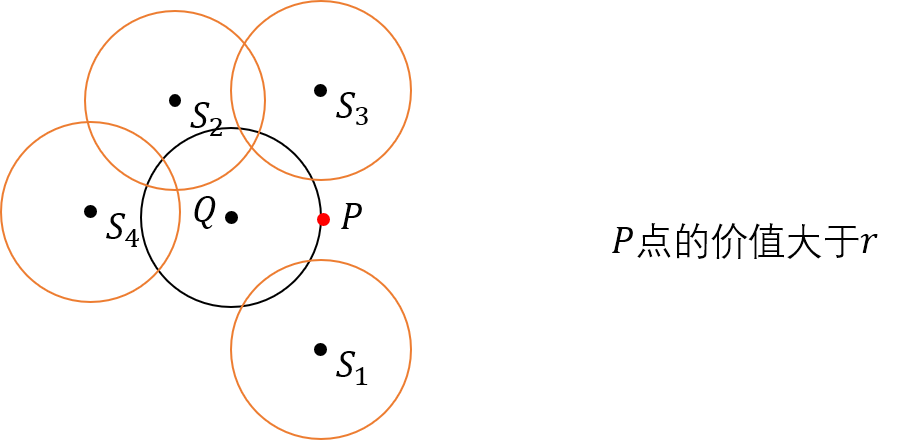
\includegraphics[width=0.8\textwidth]{pic/cf442e.png}
    \end{figure}
    
    \pause
    把 $C(S_i,r)$ 与 $C(Q,r)$ 的交点全部求出来,按逆时针排序,
    做线段覆盖(差分法),检查是否有至多被一条线段覆盖的位置即可。

    \pause
    复杂度:二分答案、枚举 $Q$、枚举 $S_i$ 求所有交点并排序,$O(\log r \cdot n^2\log n)$
\end{frame}

\begin{frame}{[CF442E] Gena and Second Distance}
    \footnotesize
    这个复杂度过不去,考虑优化。

    \vspace{1em}\pause
    先枚举,确定某个点为 $Q$,然后二分答案 $r$,
    接下来一样的求交、排序、判定。对于
    每一个 $Q$,复杂度是 $O(\log r\cdot n\log n)$。
    
    \vspace{1em}\pause
    现在,看起来外层循环枚举 $Q$ 还有一个 $O(n)$,其实不然。
    当枚举下一个 $Q$ 时,\textbf{先判断}它的答案能否大于之前的答案 $r$,
    如果不能,则没必要在这个 $Q$ 里二分答案。

    \vspace{1em}\pause
    现在,假设以每个特殊点为 $Q$,求得的答案分别为 $r_1,...,r_n$,
    如果 $r_2,...,r_i$ 均不超过 $r_1$,我们是不会以 $2,...,i$ 为 $Q$ 点进行二分的。
    换句话说,如果我们以 $j_1,j_2,...,j_k$ 这些点为 $Q$ 进行了二分,
    那么 $r_{j_1},...,r_{j_k}$ 一定是一个严格上升子序列。

    \vspace{1em}\pause
    将一个任意序列随机打乱,其最长严格上升子序列的长度期望为 $O(\log n)$。
    因此,我们的复杂度降低到了 $O(\log r\cdot n\log^2n + n^2\log n)$,
    后面加的那个 $n^2\log n$ 是因为上面提到的 “先判断……”。
\end{frame}

\begin{frame}
    \begin{center}
        {\Huge\calligra Thank You}
    \end{center}
\end{frame}

\end{document}